% Koma class
\documentclass[a4paper, oneside]{scrartcl}   

\usepackage{a4wide}

%------------------
% language = english
\usepackage[english, german]{babel}	% Umlaute mit \"u
\usepackage[latin1]{inputenc}

% margins + Kopf- und Fu�zeilen
\usepackage[left = 2.5cm, right = 2.5cm, top = 2cm, bottom = 3cm]{geometry}
\usepackage{scrpage2} 
\pagestyle{scrheadings}
\clearscrheadfoot
\rehead{\headmark}
\lehead{\pagemark}
\lohead{\headmark}
\rohead{\pagemark} 


% math
\usepackage{amssymb}
\usepackage{amsmath}

% figures
\usepackage{tikz}
\usepackage{graphicx}


% section-Zaehler wird neu gesetzt:
\setcounter{section}{3}
%------------------
\author{Sascha Meiers, Martin Seeger}
\title{Exercise 5, Discrete Mathematics for Bioinformatics}
\date{Winter term 2011/2012}


\begin{document}
\maketitle

%---------------------------------------------------------------------------------------------------

\subsection{Tree decomposition}

Let $G=(V,E)$ be a graph with $V= {v_1 , \ldots, v_n}$ and $E = {V \choose 2}$. 
We'll prove that the graph's tree width is $n-1$, meaning that any tree decomposition of $G$ 
contains at least one piece with $n$ elements.

\paragraph{Proof:} 
Given a tree decomposition $T$, let $V^*$ be the largest piece and assume that $v_n \notin V^*$ 
without loss of generality. We know by edge coverage property that there must be pieces containing 
$v_n$ and $v_i$ at the same time, for $1 \leq i \leq n-1$. Let these edges be covered by the $k$ pieces
$V_1, \ldots, V_k$ with $2 \leq k \leq n-1$ (but there could also be other pieces). $k$ cannot be one since 
then $V_k$ would be larger than $V^*$.

Now we analyze the structure of the tree $T$ and regard two cases:
\begin{enumerate}
\item The piece $V^*$ is somewhere ''between'' the pieces $V_i$.
        This means, there is at least one pair $(i,j)$ such that $V^*$ lies on a path from $V_i$ to $V_j$.
        $V_i$ and $V_j$ both contain $v_n$, but $V^*$ does not. This hurts the coherence property $\Rightarrow$ contradiction   
\item The piece $V^*$ is not between the pieces $V_i$. It could be a leaf of the tree, 
        but there could also be further pieces connected to it. However, $V^*$ is connected 
        to the subtree that contains all $V_i$ by a single edge.
        Let $X$ be the next piece on the path from $V^*$ to any $V_i$. 
        Usually\footnote{$X$ can contain at most $n-1$ nodes, so at least one node is missing, as stated. 
            Theoretically, the missing node could be $v_n$. But in this case, we have $X = V^*$ and 
            (if this is allowed at all) the argumentation (case 1 or 2) can be applied on $X$ itself as the largest set. }
        the piece $X$ is missing at least one node $v_l \neq v_n$. We know that there is at least one piece
        $V_r$ in the subtree that contains $v_l$, and we also know $v_l \in V^*$. By coherence property, 
        $X$ would also have to contain $v_l \Rightarrow$ contradiction.
        \begin{center}
        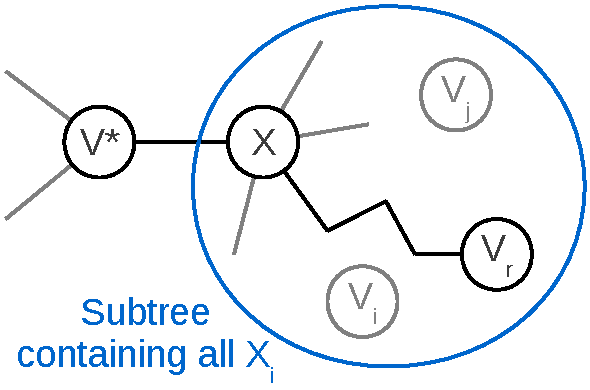
\includegraphics[width=6cm]{tree_decomposition_proof.pdf}
        \end{center}
\end{enumerate}

\end{document}
